%%%%%%%%%%%%%%%%%%%%%%%%%%%%%%%%%%%%%%%%%%%%%%%%%%%%%%%%%%%%%%%%%%%%%%%%%%%%%
% 26/05/2010
% edited by Bill Lampos
%
% Feel free to use (copy) the structure (latex formatting source code)
% but not the content of this document.
%
%%%%%%%%%%%%%%%%%%%%%%%%%%%%%%%%%%%%%%%%%%%%%%%%%%%%%%%%%%%%%%%%%%%%%%%%%%%%%
\documentclass[compress,red]{beamer}
\mode<presentation>

\usetheme{Warsaw}
% other themes: AnnArbor, Antibes, Bergen, Berkeley, Berlin, Boadilla, boxes, CambridgeUS, Copenhagen, Darmstadt, default, Dresden, Frankfurt, Goettingen,
% Hannover, Ilmenau, JuanLesPins, Luebeck, Madrid, Maloe, Marburg, Montpellier, PaloAlto, Pittsburg, Rochester, Singapore, Szeged, classic

%\usecolortheme{lily}
% color themes: albatross, beaver, beetle, crane, default, dolphin, dov, fly, lily, orchid, rose, seagull, seahorse, sidebartab, structure, whale, wolverine

%\usefonttheme{serif}
% font themes: default, professionalfonts, serif, structurebold, structureitalicserif, structuresmallcapsserif

% pdf is displayed in full screen mode automatically
%\hypersetup{pdfpagemode=FullScreen}

% define your own colours:
\definecolor{Red}{rgb}{1,0,0}
\definecolor{Blue}{rgb}{0,0,1}
\definecolor{Green}{rgb}{0,1,0}
\definecolor{magenta}{rgb}{1,0,.6}
\definecolor{lightblue}{rgb}{0,.5,1}
\definecolor{lightpurple}{rgb}{.6,.4,1}
\definecolor{gold}{rgb}{.6,.5,0}
\definecolor{orange}{rgb}{1,0.4,0}
\definecolor{hotpink}{rgb}{1,0,0.5}
\definecolor{newcolor2}{rgb}{.5,.3,.5}
\definecolor{newcolor}{rgb}{0,.3,1}
\definecolor{newcolor3}{rgb}{1,0,.35}
\definecolor{darkgreen1}{rgb}{0, .35, 0}
\definecolor{darkgreen}{rgb}{0, .6, 0}
\definecolor{darkred}{rgb}{.75,0,0}

\xdefinecolor{olive}{cmyk}{0.64,0,0.95,0.4}
\xdefinecolor{purpleish}{cmyk}{0.75,0.75,0,0}

\useoutertheme[subsection=false]{smoothbars}

\usepackage[T1]{fontenc}
\usepackage[utf8]{inputenc}
\usepackage[francais]{babel}

\usepackage{listings}
\usepackage{graphicx}
\usepackage{url}
\usepackage{hyperref}
\usepackage{subfigure}

\lstset{
  %backgroundcolor=\color{white},   % choose the background color; you must add \usepackage{color} or \usepackage{xcolor}
  basicstyle=\footnotesize,        % the size of the fonts that are used for the code
  breakatwhitespace=false,         % sets if automatic breaks should only happen at whitespace
  breaklines=true,                 % sets automatic line breaking
  %captionpos=b,                    % sets the caption-position to bottom
  %commentstyle=\color{mygreen},    % comment style
  %deletekeywords={...},            % if you want to delete keywords from the given language
  %escapeinside={\%*}{*)},          % if you want to add LaTeX within your code
  extendedchars=true,              % lets you use non-ASCII characters; for 8-bits encodings only, does not work with UTF-8
  frame=single,	                   % adds a frame around the code
  keepspaces=true,                 % keeps spaces in text, useful for keeping indentation of code (possibly needs columns=flexible)
  %keywordstyle=\color{blue},       % keyword style
  %language=Octave,                 % the language of the code
  %otherkeywords={*,...},           % if you want to add more keywords to the set
  %numbers=left,                    % where to put the line-numbers; possible values are (none, left, right)
  %numbersep=5pt,                   % how far the line-numbers are from the code
  %numberstyle=\tiny\color{mygray}, % the style that is used for the line-numbers
  %rulecolor=\color{black},         % if not set, the frame-color may be changed on line-breaks within not-black text (e.g. comments (green here))
  showspaces=false,                % show spaces everywhere adding particular underscores; it overrides 'showstringspaces'
  showstringspaces=false,          % underline spaces within strings only
  showtabs=false,                  % show tabs within strings adding particular underscores
  stepnumber=2,                    % the step between two line-numbers. If it's 1, each line will be numbered
  %stringstyle=\color{mymauve},     % string literal style
  tabsize=2,	                   % sets default tabsize to 2 spaces
  %title=\lstname                   % show the filename of files included with \lstinputlisting; also try caption instead of title
}

\title{Deboguage natif de code OCaml}
\author{Elias Boutaleb}
\institute{OCamlPro}
\date{\today}

\AtBeginSection[]
{
    \begin{frame}
     \tableofcontents[currentsection]
    \end{frame}
}

\begin{document}

\frame{
	\titlepage
}

% le contenu de la presentation va etre dense
%je coupe la partie sur la societe
\frame{\tableofcontents}

\section{Introduction}
\subsection{Pourquoi?}
\frame{\frametitle{Pourquoi du déboguage natif?}

\vspace{0.25cm}
\begin{itemize}
%oui je sais si possible deboguez votre code sans opts/en bytecode mais un bug peut apparaitre dans du code optimisé qui n'apparait pas dans le code
%non optimisé, du pas à pas ins par ins asm ca va deux minutes mais sur une appli très grande ca ne le fait pas
\item Besoin de déboguer du code optimisé
\item Pas (encore) de solution définitive/unifiée pour déboguer du code natif OCaml
%Mark, libmonda se veut une librarie de debug natif OCaml agnostique au debugger
\end{itemize}
\vspace{0.25cm}

Pourquoi sous LLDB?

\vspace{0.25cm}
\begin{itemize}
\item Support d'OCaml inexistant
%lldb ne sait meme pas qu'il debugge un binaire OCaml
% MS s'occupe deja du support cote gdb
\item ocplib-lldb : une liaison (binding) vers lldb en OCaml
%gen auto faite en parsant les fichiers d'entetes C++, non parfaite mais une majeure partie des fonctions de l'API sont la
\item Apple préfere LLVM à la toolchain GNU
%(XCode utilise LLDB pour deboguer du ObjC et Swift)
\end{itemize}
}

\subsection{A l'heure actuelle}
\frame{\frametitle{A l'heure actuelle}
\begin{itemize}
    \item Consultation de la pile d'appels de fonction
        %directives DWARF CFI permettent de la reconstruire
    \item Pas à pas partiel aux points d'entrée et d'appel de fonctions
        %consequence du patch de thomasg qui propage les debug events du BC vers le backend natif
\end{itemize}
}

\subsection{Objectifs du stage}
\frame{\frametitle{Objectifs du stage}

Développer/améliorer le prototype de débogueur natif OCaml : ocp-lldb
\begin{enumerate}
    \item Modifier le compilateur pour générer plus d'informations de déboguage
        % emplacement des variables en memoire, correspondance entre instruciton asm et une ligne du code source
        % info sous forme lisible par LLDB
    \item Implanter les opérations classiques d'un débogueur
        % en utilisant les infos generes depuis le compilateur
        % affichage des valeurs de variables, pas a pas dans la source
\end{enumerate}
}

\section{DWARF}

%transition
% logique derriere deboguage au niveau du code source
% - code asm ne conserve aucune des abstractions presentes dans le code source, ni dans l'AST, les IRs, aucun type
% - optimisations peuvent transformer/deplacer des parties de code a travers le programme
% - implique de grosses pertes d'information
%pour pouvoir etablir correspondance entre source et code machine, on veut pouvoir
% collecter toutes les infos utilisees dans la transformation du code source passe a un compilateur
% (pblm : au niveau du backend, le code manipule peut ne plus rien a voir avec le code source d'origine) - si gen des info dbg
%a ce niveau)
% representer ces donnes dans un format adequat, de maniere concise et compacte, et suffisamment de details

\subsection{Présentation de DWARF}
\frame{\frametitle{Présentation de DWARF (1)}

%\begin{exampleblock}{This is an Example block}
%This is an example
%\end{exampleblock}

\begin{columns}
    \begin{column}{0.48\textwidth}
        \centering
        
\includegraphics[width=0.5\textwidth]{dwarf.png}%
    \end{column}
    \begin{column}{0.48\textwidth}
        \centering
        
\includegraphics[width=0.5\textwidth]{df2.png}
    \end{column}
\end{columns}

\begin{itemize}
\item Format d'information de données de déboguage
\item Agnostique au language de programmation
\item Agnostique aux compilateurs, assembleurs et debogueurs
% fichier objet = code + metadata pour linking/debug/profile/stack unwind/relocation
\item Agnostique au format de fichier objet
 %(même si utilisé le plus souvent avec ELF)
\item Standardisé et extensible
% un comité receuille propositions d'extensions du std, mnt DWARF4
\end{itemize}
}

\frame{\frametitle{Présentation de DWARF (2)}

Chaque type de données est placé dans une section dédiée dans le binaire

%je passe sur la repr binaire du format dwarf
%j'expose ici les sections DWARF les plus importantes pour un debogueur

\begin{itemize}
\item .debug\_info: contient les informations principales DWARF
\item .debug\_abbrev: abbreviations (signatures) utilisées pour décoder .debug\_info
% decrivent forme des records utilises dans debug_info
\item .debug\_loc: listes de locations (emplacement des variables à l'exécution)
% sur la pile (et dans le cas, quel offset),  dans un registre
\item .debug\_line: table des numéros de ligne dans la source
% etablit correspondance entre adresses memoires du code executable et les lignes du code source
\end{itemize}

}

\frame{\frametitle{Une section importante : .debug\_info}

\begin{itemize}
\item \item Entité de base : le DIE (Debugging Information Entry)
%entree d'info de debug
\item DIE = un tag + ensemble d'attributs
\item Un tag spécifie ce que le DIE represente (variable, portée lexicale, fonction, type)

\item Un attribut = couple de clé/valeur
%(fst décrit ce qui est repr - un nom, une adresse, snd une valeur (peut etre un nombre, offset, adresse)
\item Peut referencer d'autres entrées voire d'autres sections

\item les DIES peuvent etre imbriques dans d'autres DIES, formant une structure d'arbre
\item Racine est une unité de compilation (CU) <=> un fichier source compilé /objet
%\item Compilation séparée : mise en commun des sections DWARF dans des sections communes au binaire final (linker)

\end{itemize}
}


\subsection{Exemple}
\frame{\frametitle{Exemple}
\lstinputlisting[language=C, firstline=3, lastline=14]{d.c}
}

\frame{\frametitle{Arbre d'entrées}
\centering
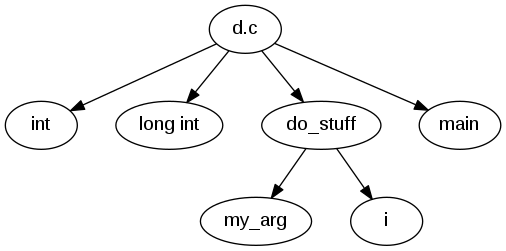
\includegraphics[width=0.85\textwidth]{test.png}
}

\frame{\frametitle{Exemple (2)}
\lstinputlisting[firstline=11, lastline=18]{dwarf}
}

\frame{\frametitle{Exemple (3)}
\lstinputlisting[firstline=43, lastline=50]{dwarf}
}

\frame{\frametitle{Exemple (4)}
\lstinputlisting[firstline=59, lastline=69]{dwarf}
}

% call_frame_cfa : retrieve cfa frame base location from debug_frame section
\frame{\frametitle{Exemple (5)}
\lstinputlisting[firstline=70, lastline=82]{dwarf}
}

% vous pouvez voir que ce format n'est pas sense etre lu par des humains

\subsection{ocp-dwarf}
\frame{\frametitle{ocp-dwarf}
\begin{itemize}
\item Bibliothèque de lecture et d'affichage d'informations DWARF
%sortie similaire a objdump
\item Offre une abstraction permettant de manipuler les structures de données%
\item Ecriture et édition restent à faire
% meme si cette tache est deleguee aux compilateurs
\end{itemize}
}

%transition : le format dwarf semble ideal pour stocker les infos de debug
%sa complexite est telle qu'il peut decrire du C++

\section{Ajouts faits au compilateur natif}
\subsection{Propagation des évenements de déboguage}
\frame{\frametitle{Propagation des évenements de déboguage (1)}
\begin{enumerate}
\item Problème : pas à pas dans le code source
\item Necessaire aussi pour poser des breakpoints suivant fichier/num de ligne

%Comment?
% dans le code assembleur, présence de directives .loc
%fichier - num de ligne - num de colonne
%assembleur recupere les infos et l'offset et encode tout cela dans une structure dediée dans la section .debug\_line
\end{enumerate}
}

\frame{\frametitle{Propagation des évenements de déboguage (2)}
\begin{enumerate}
\item Idée : le bytecode ocaml contient des évenements de débug
    %(info de num de ligne/colonne/fichier)
%\item Necessaire aussi pour poser des points d'arrêt suivant fichier/num de ligne
\item Patch de Thomas Gazagnaire propage ces informations à travers le backend
% patch porte de 3.12.1 a 4.02.1
Inconvénients :

\begin{enumerate}
\item Modifications lourdes au compilateur
\item Manque de précision, perte d'informations
% code subit encore des transformations/optimisations, est expansé puis réduit
\item Valeurs disponibles pas toujours cohérentes
\end{enumerate}

\end{enumerate}
}

\subsection{Emetteur DWARF}
\frame{\frametitle{Emetteur DWARF}
\begin{itemize}
\item Fourni et développé par Mark Shinwell (Jane Street)
\item Recupere les let-bindings presents dans les definitions de structures toplevel du module
\item Deux passes supplémentaires dans le backend: available\_regs et available\_ranges
% emploie tech d'analyse de flot de donnees en avant
% available\_regs parcourt le CFG Mach d'une fonction et determine pour chaque ins manip  l'ens des regs avec un ident "disponibles",
%cad dont la valeur peut etre inspectee par un debuggeur
% available_ranges determine pour chaque variable/identifieur d'une fonction les intervalles ou sa valeur est disponible,
% et pour chaque intervalle, le registre qui contient sa valeur
\item ne capture pas les value bindings victimes d'optimisations
% cst folding - reduction de constantes
% Mark veut y remedier avec des let fantomes dans flambda
%id unique conservé en cas de masquage de variable
\end{itemize}
}

%\subsection{Informations de type}
%\frame{\frametitle{Informations de type}
%\begin{enumerate}
      %\begin{itemize}
        %\item Predict flu rates (\emph{epidemics})
        %\item Infer vote intensions (\emph{politics})
        %\item Infer traffic/weather conditions (\emph{toy problems})
            %\pause
      %\end{itemize}
%\vspace{0.25cm}
%\item \textbf{Methodologies}?
      %\begin{itemize}
        %\item Feature extraction/selection
        %\item Exploit probabilistic relationships (PGMs)
        %\item Regression/classification/ranking scenarios
        %\item Active learning
      %\end{itemize}
%\end{enumerate}
%}

\section{Déboguage sous LLDB}
\subsection{Plugin LLDB}
\frame{\frametitle{Plugin LLDB}
\begin{enumerate}
\item A ce stade, le binaire contient plus d'informations... \pause

%plus d'endroits ou poser un point d'arrêt
\item ...qui ne peuvent pas etre lues par LLDB \pause
% DWARF emis pas structure comme celui de C/C++, et
% LLDB croit qu'il debugge du C
\item Maintenant possible d'ajouter d'autres languages à LLDB
% depuis un peu moins d'un an, chgmts faits a LLDB pour pouvoir supporter d'autres languages que ceux supportes par clang
% il suffit d'ecrire des classes impl des interfaces precises
% ajouter le language cible dans un enum

% eventuellement pouvoir evaluer expr dans ce language
% pretty printing des valeurs et typage dynamique, ptes statiques ou dyn du language
\end{enumerate}
}

\frame{\frametitle{Plugin LLDB (2)}
\begin{enumerate}
\item Parseur DWARF
\item Système de type minimal
%(toutes les valeurs sont des entiers 64 bits, leur eval est laissee a ocp-lldb)
\item Démanglage des symboles
\end{enumerate}
}

\subsection{ocp-lldb}
\frame{\frametitle{ocp-lldb}
\begin{enumerate}
\item Intégration de nouvelles commandes lldb en OCaml
%structure des noeuds de l'ast/typedtree, types peuvent changer d'une version du compilateur a une autre
\item Table de symboles
\item Récuperer le type associé à une variable et afficher sa valeur
\end{enumerate}
}

\frame{\frametitle{Démonstration}
}


% amelioration
%commande qui liste les endroits ou un bp peut etre place?

\section*{Conclusion}

\frame{\frametitle{Etat actuel du projet}
\begin{enumerate}
\item Systèmes visés: Linux x86 64 bits
\item Plupart des outils encore non disponible au public
% présenté
% en particulier le fork du compilateur avec support pour profiling memoire
% devrait etre mis a disposition au public dans un futur plus ou moins proche
% partie emission DWARF de MS et deboguage natif: peut etre pour 4.05
\item Plugin LLDB OCaml et ocp-dwarf peuvent être rendus disponible
% pour peu que la PR soit soumise
% mais modifications moins maintenables et touchant plus au debugger lui meme que le plugin
% compilateur reste a reste modifie en consequence
\item ocp-lldb déjà disponible
%mais necessite fork avec memprof
%la branche sur laquelle je travaille necessite un autre fork encore avec mes ajouts
\item Augmenter le nombre de dbg events/locations
% chronophage car precision de methode naive + temps de compilation de la compiler suite
\end{enumerate}
}

\frame{\frametitle{Fin}
    \begin{center}
        \huge
        Des questions?
    \end{center}
}

\end{document}
